\ifdefined\included
\else
\documentclass[english,a4paper,11pt,twoside]{StyleThese}
\usepackage{amsmath,amssymb}             % AMS Math
\usepackage[T1]{fontenc}
\usepackage[utf8x]{inputenc}
\usepackage{babel}
\usepackage{datetime}

\usepackage{lmodern}
\usepackage{tabularx}
%\usepackage{tabular}
\usepackage{multirow}

\usepackage{subfigure}
\usepackage{fancyvrb}


\usepackage{hhline}
\usepackage[left=1.5in,right=1.3in,top=1.1in,bottom=1.1in,includefoot,includehead,headheight=13.6pt]{geometry}
\renewcommand{\baselinestretch}{1.05}

% Table of contents for each chapter

\usepackage[nottoc, notlof, notlot]{tocbibind}
\usepackage{minitoc}
\setcounter{minitocdepth}{2}
\mtcindent=15pt
% Use \minitoc where to put a table of contents

\usepackage{aecompl}


% Glossary / list of abbreviations

\usepackage[intoc]{nomencl}
\iftoggle{ThesisInEnglish}{%
\renewcommand{\nomname}{Glossary}
}{ %
\renewcommand{\nomname}{Liste des Abréviations}
}

\makenomenclature

% My pdf code

\usepackage{ifpdf}

\ifpdf
  \usepackage[pdftex]{graphicx}
  \DeclareGraphicsExtensions{.jpg}
  \usepackage[a4paper,pagebackref,hyperindex=true]{hyperref}
  \usepackage{tikz}
  \usetikzlibrary{arrows,shapes,calc}
\else
  \usepackage{graphicx}
  \DeclareGraphicsExtensions{.ps,.eps}
  \usepackage[a4paper,dvipdfm,pagebackref,hyperindex=true]{hyperref}
\fi

\graphicspath{{.}{images/}}

%% nicer backref links. NOTE: The flag ThesisInEnglish is used to define the
% language in the back references. Read more about it in These.tex

\iftoggle{ThesisInEnglish}{%
\renewcommand*{\backref}[1]{}
\renewcommand*{\backrefalt}[4]{%
\ifcase #1 %
(Not cited.)%
\or
(Cited in page~#2.)%
\else
(Cited in pages~#2.)%
\fi}
\renewcommand*{\backrefsep}{, }
\renewcommand*{\backreftwosep}{ and~}
\renewcommand*{\backreflastsep}{ and~}
}{%
\renewcommand*{\backref}[1]{}
\renewcommand*{\backrefalt}[4]{%
\ifcase #1 %
(Non cité.)%
\or
(Cité en page~#2.)%
\else
(Cité en pages~#2.)%
\fi}
\renewcommand*{\backrefsep}{, }
\renewcommand*{\backreftwosep}{ et~}
\renewcommand*{\backreflastsep}{ et~}
}

% Links in pdf
\usepackage{color}
\definecolor{linkcol}{rgb}{0,0,0.4} 
\definecolor{citecol}{rgb}{0.5,0,0} 
\definecolor{linkcol}{rgb}{0,0,0} 
\definecolor{citecol}{rgb}{0,0,0}
% Change this to change the informations included in the pdf file

\hypersetup
{
bookmarksopen=true,
pdftitle="Joint Action for Human-Robot Interaction",
pdfauthor="Sandra DEVIN", %auteur du document
pdfsubject="Thesis", %sujet du document
%pdftoolbar=false, %barre d'outils non visible
pdfmenubar=true, %barre de menu visible
pdfhighlight=/O, %effet d'un clic sur un lien hypertexte
colorlinks=true, %couleurs sur les liens hypertextes
pdfpagemode=None, %aucun mode de page
pdfpagelayout=SinglePage, %ouverture en simple page
pdffitwindow=true, %pages ouvertes entierement dans toute la fenetre
linkcolor=linkcol, %couleur des liens hypertextes internes
citecolor=citecol, %couleur des liens pour les citations
urlcolor=linkcol %couleur des liens pour les url
}

% definitions.
% -------------------

\setcounter{secnumdepth}{3}
\setcounter{tocdepth}{2}

% Some useful commands and shortcut for maths:  partial derivative and stuff

\newcommand{\pd}[2]{\frac{\partial #1}{\partial #2}}
\def\abs{\operatorname{abs}}
\def\argmax{\operatornamewithlimits{arg\,max}}
\def\argmin{\operatornamewithlimits{arg\,min}}
\def\diag{\operatorname{Diag}}
\newcommand{\eqRef}[1]{(\ref{#1})}

\usepackage{rotating}                    % Sideways of figures & tables
%\usepackage{bibunits}
%\usepackage[sectionbib]{chapterbib}          % Cross-reference package (Natural BiB)
%\usepackage{natbib}                  % Put References at the end of each chapter
                                         % Do not put 'sectionbib' option here.
                                         % Sectionbib option in 'natbib' will do.
\usepackage{fancyhdr}                    % Fancy Header and Footer

% \usepackage{txfonts}                     % Public Times New Roman text & math font
  
%%% Fancy Header %%%%%%%%%%%%%%%%%%%%%%%%%%%%%%%%%%%%%%%%%%%%%%%%%%%%%%%%%%%%%%%%%%
% Fancy Header Style Options

\pagestyle{fancy}                       % Sets fancy header and footer
\fancyfoot{}                            % Delete current footer settings

%\renewcommand{\chaptermark}[1]{         % Lower Case Chapter marker style
%  \markboth{\chaptername\ \thechapter.\ #1}}{}} %

%\renewcommand{\sectionmark}[1]{         % Lower case Section marker style
%  \markright{\thesection.\ #1}}         %

\fancyhead[LE,RO]{\bfseries\thepage}    % Page number (boldface) in left on even
% pages and right on odd pages
\fancyhead[RE]{\bfseries\nouppercase{\leftmark}}      % Chapter in the right on even pages
\fancyhead[LO]{\bfseries\nouppercase{\rightmark}}     % Section in the left on odd pages

\let\headruleORIG\headrule
\renewcommand{\headrule}{\color{black} \headruleORIG}
\renewcommand{\headrulewidth}{1.0pt}
\usepackage{colortbl}
\arrayrulecolor{black}

\fancypagestyle{plain}{
  \fancyhead{}
  \fancyfoot{}
  \renewcommand{\headrulewidth}{0pt}
}

%\usepackage{MyAlgorithm}
%\usepackage[noend]{MyAlgorithmic}
\usepackage[ED=MITT - STICIA, Ets=INP]{tlsflyleaf}
%%% Clear Header %%%%%%%%%%%%%%%%%%%%%%%%%%%%%%%%%%%%%%%%%%%%%%%%%%%%%%%%%%%%%%%%%%
% Clear Header Style on the Last Empty Odd pages
\makeatletter

\def\cleardoublepage{\clearpage\if@twoside \ifodd\c@page\else%
  \hbox{}%
  \thispagestyle{empty}%              % Empty header styles
  \newpage%
  \if@twocolumn\hbox{}\newpage\fi\fi\fi}

\makeatother
 
%%%%%%%%%%%%%%%%%%%%%%%%%%%%%%%%%%%%%%%%%%%%%%%%%%%%%%%%%%%%%%%%%%%%%%%%%%%%%%% 
% Prints your review date and 'Draft Version' (From Josullvn, CS, CMU)
\newcommand{\reviewtimetoday}[2]{\special{!userdict begin
    /bop-hook{gsave 20 710 translate 45 rotate 0.8 setgray
      /Times-Roman findfont 12 scalefont setfont 0 0   moveto (#1) show
      0 -12 moveto (#2) show grestore}def end}}
% You can turn on or off this option.
% \reviewtimetoday{\today}{Draft Version}
%%%%%%%%%%%%%%%%%%%%%%%%%%%%%%%%%%%%%%%%%%%%%%%%%%%%%%%%%%%%%%%%%%%%%%%%%%%%%%% 

\newenvironment{maxime}[1]
{
\vspace*{0cm}
\hfill
\begin{minipage}{0.5\textwidth}%
%\rule[0.5ex]{\textwidth}{0.1mm}\\%
\hrulefill $\:$ {\bf #1}\\
%\vspace*{-0.25cm}
\it 
}%
{%

\hrulefill
\vspace*{0.5cm}%
\end{minipage}
}

\let\minitocORIG\minitoc
\renewcommand{\minitoc}{\minitocORIG \vspace{1.5em}}

\usepackage{multirow}
%\usepackage{slashbox}

\newenvironment{bulletList}%
{ \begin{list}%
	{$\bullet$}%
	{\setlength{\labelwidth}{25pt}%
	 \setlength{\leftmargin}{30pt}%
	 \setlength{\itemsep}{\parsep}}}%
{ \end{list} }

\newtheorem{definition}{Définition}
\renewcommand{\epsilon}{\varepsilon}

% centered page environment

\newenvironment{vcenterpage}
{\newpage\vspace*{\fill}\thispagestyle{empty}\renewcommand{\headrulewidth}{0pt}}
{\vspace*{\fill}}

\usepackage{tablefootnote}

\sloppy
\begin{document}
\setcounter{chapter}{2} %% Numéro du chapitre précédent ;)
\dominitoc
\faketableofcontents
\fi

\chapter{Taking Humans Mental States into account while executing Shared Plans}
\minitoc

\label{ch:MS}

\section{Motivations}

When collaborating with humans, it is primordial for the robot to not consider humans as obstacles or tools impacting the environment. As humans are social creatures, the robot must take into account their comfort and so, their point of view. Several works already allow robots to estimate humans perspective and beliefs concerning its environment. In order to improve human-robot Joint Action, the robot must be able to take these information into account when taking decision on how to act or what to communicate. Even if several works have been done on how to integrate humans perspective in dialogue or use it to help the understanding of humans behavior, there is still a gap when it came to use it during Shared Plan execution. This work aims to start filling this gap by extending the robot knowledge on humans mental states to the joint task and using it to better communicate during Shared Plan execution. It has been the subject of a publication into the HRI conference \cite{devin2016implemented}.

\section{Theory of Mind}

\subsection{Social Sciences literature}

Theory of the Mind (ToM) refers to the ability humans have to recognize and attribute mental states not only to themselves but to other people, to understand that feelings and beliefs we have may be different than others and to take others mental states into account. ToM has been deeply studied in psychology, notably in the developmental domain \cite{baron1985does, premack1978does}. \cite{verbrugge2008learning} defines what is called "order" of ToM:
\begin{quote}
"To have a first-order ToM is to assume that someone’s beliefs,
thoughts and desires influence one’s behavior. A first-order thought could be: ‘He does not know that his book is on the table’. In second-order ToM it is also recognized that to predict others’ behavior, the desires and beliefs that they have of one’s self and the predictions of oneself by others must be taken into account. So, for example, you can realize that what someone expects you to do will affect his behavior. For example, ‘(I know) he does not know that I know his book is on the table’ would be part of my second-order ToM. To have a third-order ToM is to assume others to have a second-order ToM, etc."
\end{quote}
There is an infinitesimal numbers of orders, however, studied shown that orders above the second one do not help in cooperative tasks \cite{de2014theory} and above the third one do not help for competitive games \cite{de2014theory}.


\begin{figure*}[!h]
    \centering
    \subfigure[Perceptual perspective taking: two individuals can have a different representation of their environment considering their locations.]{
        \centering
        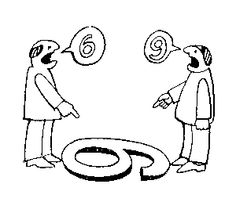
\includegraphics[width=0.4\textwidth]{figs/Chapter3/perceptual.jpg}
       \label{subfig:perceptual}
   }
    %~
    \subfigure[Conceptual perspective taking: here Bob attributes to Alice a belief concerning the box. He thinks Alice thinks the box is empty.]{
        \centering
        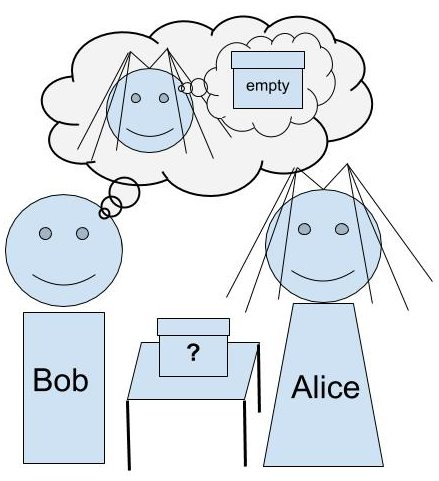
\includegraphics[width=0.4\textwidth]{figs/Chapter3/conceptual.jpg}
       \label{subfig:conceptual}
    }
    \caption{Illustration of perceptual and conceptual perspective taking.}
\end{figure*}

ToM includes the notion of perspective taking: the capacity for a person to reason by taking the point of view of someone else. Studied in literature \cite{tversky1999speakers, flavell1992perspectives}, perspective taking is crucial during humans interaction and studies have demonstrate that individuals who lack of this ability have difficulties in their daily social interactions \cite{frick2014picturing}. Two levels of perspective taking are defined in \cite{flavell1977development}: perceptual and conceptual perspective taking. Perceptual perspective taking design the capacity of a person to understand that others have a different perception of the world (fig~\ref{subfig:perceptual}). Conceptual perspective taking designs the capacity of a person to attribute beliefs and feelings to others (fig~\ref{subfig:conceptual}).

\begin{figure}[!h]
	\centering
    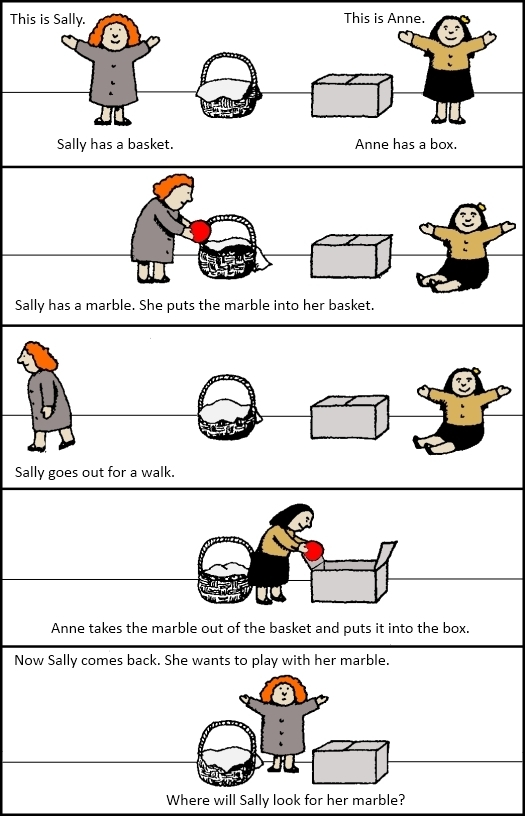
\includegraphics[width=0.7\textwidth]{figs/Chapter3/sally.jpg}
    \caption{The Sally and Anne test: it allows to check the capacity of someone to attribute a false-belief to another person. Illustration from the work of Axel Scheffler.}
    \label{fig:sally}
\end{figure}

To check if an individual has ToM capacities, several tests have been developed in psychology. One of the most famous is the Sally and Anne test (fin~\ref{fig:sally}). This test allows to check the capacity of someone to attribute a false-belief to another person and have been reused in robotics to validate perspective taking systems.

\subsection{Robotics background}

One of the pioneer work in robotics Theory of Mind is \cite{scassellati2002theory}. Scassellati presents two models from social sciences (Leslie \cite{leslie1984spatiotemporal} et Baron-Cohen \cite{baron1997mindblindness}) and proposes a model on how to implement ToM in robotics. However, the implementation of this model did not go further than perception level.

Then, several works have been done in order to endow robots with perspective taking abilities. Using ACT-R architecture \cite{anderson2004integrated}, the team of Hiatt and Trafton models mechanisms used during the Sally and Anne test and constructs a model that learns to deal with false belief to pass this test \cite{hiatt2010cognitive}. They extend this work to second-order in \cite{hiatt2015understanding} and to spatial reasoning in \cite{hiatt2004cognitive}. The Sally and Anne test has also been passed in \cite{milliez2014framework} where the robot constructs a semantic representation of the world from its partners point of view. In \cite{berlin2006perspective}, authors present a way to record different beliefs of other agents and so to have a memory of perspective taking. Finally, \cite{johnson2005perspective} presents a system which computes perspective taking perspective taking based on forward and inverse visual models.

Perspective taking abilities have been used in robotics for several purposes. It has been used in \cite{hiatt2011accommodating} to deal with uncertainty in humans behavior and in \cite{ros2010solving} to solve ambiguous references to an object. One important application of perspective taking is action recognition. \cite{johnson2005perceptual} takes the visual point of view of humans to improve action recognition, Dynamic Bayesian Networks (DBN) are used in \cite{baker2014modeling} or inverse reinforcement learning  in \cite{nagai2015probabilistic}. The human perspective is also used in \cite{breazeal2006using} to learn a task from a situation that can be ambiguous from the robot point of view and in \cite{gray2014manipulating} to choose actions with the adequate effects in order to manipulate humans mental models. Finally, \cite{gorurtoward} uses perspective taking to infer humans intention and adapt robot decision.

Concerning Shared Plans, they can be found by using perspective taking in order to add communication actions \cite{guitton2012belief}. Then, the human perspective is used to share the plan with a level of details depending of human knowledge \cite{milliez2016using}. However, there is no works for now concerning the management of Shared Plans execution taking into account the human point of view. 

\section{Estimating Humans Mental States}

\begin{itemize}
\item reminder representation, estimate operator
\item world state: observable and non-observable
\item goal
\item Shared Plan, Actions
\end{itemize}

\section{Mental States for Shared Plans execution}

\begin{itemize}
\item solve db operator
\item weak achievement goal
\item human should act
\item preventing mistakes
\item robot action signalling
\item inaction and uncertainty
\end{itemize}

\section{Results}

\subsection{Tasks}

\begin{itemize}
\item clean the table
\item inventory
\end{itemize}

\subsection{Interesting scenario}

Clean the table ICSR paper

\subsection{Experiment and results}

\begin{itemize}
\item in simulation
\item human follows hatp plan, human leaves
\item criteria
\item results
\item discussion
\end{itemize}

\ifdefined\included
\else
\bibliographystyle{StyleThese}
\bibliography{These}
\end{document}
\fi
